In this chapter, we provide detailed information regarding the design of the framework, as well as its implementation.

\section{Basics}

The modular framework, to which we called BlockLearning, is designed in such a way that modules can be added, as well as removed or changed, easily. In this framework, the devices, identified by the address of their account in the blockchain, can be classified into three categories: \textit{trainers}, \textit{aggregators} and \textit{scorers}. Additionally, the entity that deploys the contract and is responsible for starting and terminating the rounds is called \textit{owner}.

A device can be categorized as one or more categories. By doing so, the framework provides flexibility to support different architectures and algorithms. For example, BlockFlow's scoring algorithm is done at the clients, which are then categorized as trainers and scorers, while the servers are categorized as aggregators. In contrast, Multi-KRUM is executed at the servers, which are then categorized as aggregators and scorers, while the clients are categorized as trainers.

The following sections present the execution flow of the framework, as well as the structure and modules of BlockLearning.

\section{Execution Flow}\label{meth:exec_flow}

\begin{figure}[!ht]
    \centering
    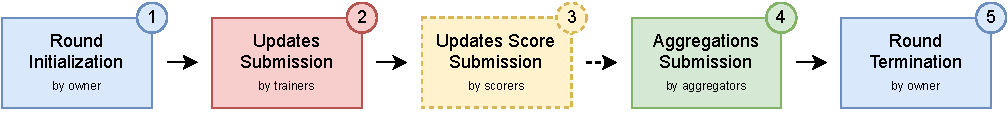
\includegraphics[width=1\textwidth]{graphics/sequence.pdf}
    \caption{BlockLearning Flow}
    \label{fig:blocklearning_steps}
\end{figure}

The framework supports a modular sequential flow represented on \autoref{fig:blocklearning_steps}. The steps are explained below:

\begin{enumerate}
    \item In first place, the owner initializes the round. During the round initialization, depending on the participant selection algorithm, the trainers that will participate may have been selected already, or not.
    
    \item In second place, the trainers retrieve the information about the round, such as the global weights from the last round, and train the model using their local data. Then, the trainers submit their updates.
    
    \item In third place, if there is a scoring algorithm enabled, the scorers retrieve the updates and calculate the scores. Then, they submit their scores.
    
    \item In fourth place, the aggregators retrieve the updates and execute the aggregation algorithm and submit the aggregation results.
    
    \item In fifth place, if we are using vertically partitioned data, and depending on the model in use, the trainers may have to confirm back-propagation. Note that this step is tightly connected to the model we will be using for Vertical Federated Learning, which will be introduced later. Nonetheless, it shows how modular the system can be and how steps can be easily added at different points of the flow for different purposes.
    
    \item Finally, the round is marked as terminated by the owner. At this point, the smart contract decides which is the final aggregation for the model based on the submissions by the aggregators.
\end{enumerate}

\section{Threat Model}

In the last step of the execution flow, the smart contract decides the final aggregation values based on the submissions by the aggregators. For this, at least 50\% of the aggregators must agree on the same aggregation in order for it to be accepted. Therefore, the framework offers a 50\% threat model.

Even though 50\% is not the ideal threat model, it is an improvement compared to classic FL where the central aggregator is a central point of failure that needs to be available, reliable and trusted at all times. In this framework, an attacker would have to control over 51\% of the servers in order to be able to influence the outcome of the aggregation, and therefore, or the training.

In addition, the framework should allow for the threat threshold to be changed. By default, it is 50\%. However, if a user prefers that all aggregators must agree on the same aggregation, they should be able to do so.

\section{Structure and Modules}\label{meth:struct_modules}

The framework is divided into three main components: the smart contracts, the library and the testbed. These are depicted on \autoref{fig:blocklearning_modules} and will be individually explored on the following subsections.

\begin{figure}[!ht]
    \centering
    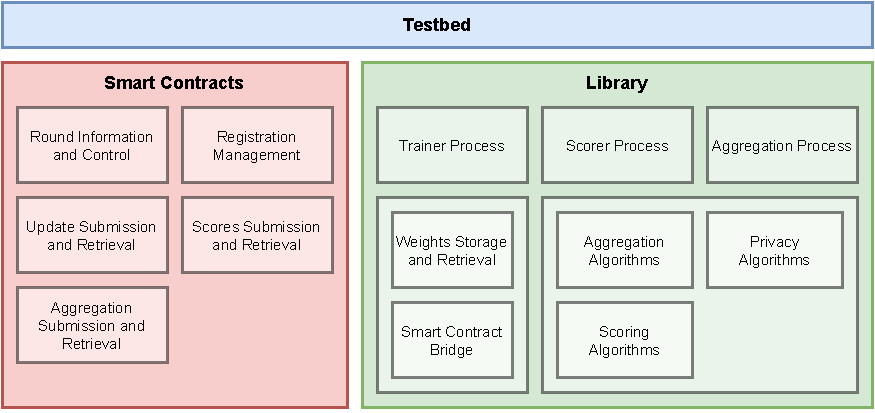
\includegraphics[width=1\textwidth]{graphics/modules.pdf}
    \caption{BlockLearning Structure and Modules}
    \label{fig:blocklearning_modules}
\end{figure}

\section{Smart Contracts}\label{meth:smart_contracts}

The first component of the framework is the smart contracts. The smart contracts live on the blockchain and are the main means of communication between clients and servers. In addition, the smart contracts hold information regarding the current status of the round, as well as the updates, scores, aggregations, among others. The smart contracts provide the following functionality:

\begin{itemize}
    \item \textit{Round Information and Control}: the smart contract must provide information on whether the round is ongoing and which phase it is in: scoring, aggregation or termination. It must allow for flexibility such that new phases can be added in the future. In addition, it must allow for rounds to be started and marked as terminated. Round phase advancements are defined through pre-defined conditions that, once met, automatically move the round to the next phase. For example, after all updates are received, the smart contract should move to the next phase.
    
    \item \textit{Registration Management}: the smart contract must allow devices to register themselves as trainers, aggregators, or scorers in the system. Regarding the owner, it is automatically assigned to whom deployed the contract. Finally, it should provide information about which devices participate in each round.
    
    \item \textit{Update Submission and Retrieval}: the smart contract must allow trainers to submit their updates, which must include a pointer to the model weights and the amount of data points that were used to train the model. In addition, it can include the training accuracy and testing accuracy for each individual trainer. The submissions must be accessible.
    
    \item \textit{Scores Submission and Retrieval}: the smart contract must allow scorers to submit their scores. It must be possible to know which scorer scored which update and they must be accessible.
    
    \item \textit{Aggregation Submission and Retrieval}: the smart contract must allow aggregators to submit the aggregations, which contain a pointer to the weights. The aggregations must be accessible.
\end{itemize}

\section{Library}\label{meth:library}

The second component of the framework is the library. The library encodes the algorithms, utilities and building blocks necessary to write the process that runs on the clients and the servers. It must include:

\begin{itemize}
    \item \textit{Aggregation, Scoring} and \textit{Privacy Algorithms}: provide implementation for aggregation, scoring and privacy algorithms. Each of these categories of algorithm must implement a common interface, such that adding new algorithms is easy and simple and they are interchangeable in the code.
    
    \item \textit{Weights Storage and Retrieval}: utilities to load and store weights on the decentralized storage provider. These must also provide an interface in order to make it easy to change the storage provider by providing a different implementation.
    
    \item \textit{Smart Contract Bridge}: a contract class that provides an interface to the smart contract that lives on the blockchain. With this class, it should be possible to call the smart contract functions as if they were local functions.
    
    \item \textit{Trainer, Scorer} and \textit{Aggregator Classes}: a class per each device category. This class must register the devices as their category upon initialization. It must also provide methods to execute the training, scoring and aggregation tasks, respectively.
\end{itemize}

\section{Testbed}\label{meth:testbed}

The third component of the framework is the testbed. The testbed provides the platform to conduct the experiments in a reproducible way. It must include:

\begin{itemize}
    \item \textit{Client} and \textit{Server Processes}: scripts that will be run at the clients and the servers, respectively. These scripts will use the library in order to perform the right tasks according to which algorithm is being used.
    
    \item \textit{Federated Learning Setup and Deployment}: scripts and tools to easily deploy the client and server machines in a test environment, such as containers.
    
    \item \textit{Blockchain Setup and Deployment}: scripts and tools to easily deploy the blockchain network in a test environment, as well as deploy the contract to such network.
\end{itemize}

In addition, the testbed must also include tools to collect the required statistics and logs that can be later processed to retrieve the previously discussed metrics.